\section{Bestiaire}

\subsection{Pilier de bar Horoxien} \label{sec:horoxian-barfly}
\begin{figure}[h!]
    \centering
    
\includegraphics[height=200pt]{_img/bestiary/horoxian-barfly.png}
\end{figure}
\paragraph{Background}
Pas très malin, le pilier de bar horoxian se cache dans les cantina d’Horox III. Passe le plus clair de son temps à picoler et a refaire le monde avant de retourner à sa pauvre vie dénuée d’intéret. C’est pourquoi dés que l’occasion se présente d’engager une bagarre, peu importe la raison, le pilier de bar Horoxien n’hésite pas ... Bien bourré, le pilier de bar Horoxien ne sent pas la douleur, il n’est pas géné par ses blessures.

\paragraph{Traits}

\begin{itemtable}[ c c c c c ]
    \textbf{Agi} & \textbf{Int} & \textbf{\^Ame} & \textbf{For} & \textbf{Vig} \\
    d4           & d2           & d2             & d8           & d8
\end{itemtable}
\begin{itemtable}[ l X ]
    \textbf{Allure}      & 6 \\
    \textbf{Compétences} & Combat d6
\end{itemtable}

\paragraph{Défense}
\begin{itemtable}[ c c ]
    \textbf{Parade}     & \textbf{Résistance} \\
    6                   & 6
\end{itemtable}

\paragraph{Arme possible}
\begin{itemtable}[ X c c ]
    ~                & \textbf{Dégats} \\
    Bouteille cassé  & 2d8
\end{itemtable}


\newpage

\subsection{Garde de la citadelle} \label{sec:citadel-guard}
\begin{figure}[h!]
    \centering
    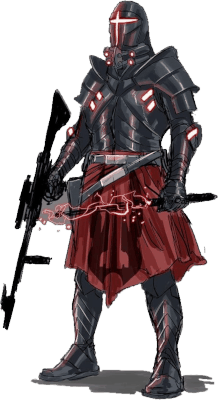
\includegraphics[height=200pt]{_img/bestiary/citadel-guard.png}
\end{figure}
\paragraph{Background}
Gardes au service de la reine. Ne parlent pas, ne réfléchissent pas et obéissent sans poser de question aux ordres de \nameref{sec:bombinax}. Formés au combat depuis leur plus tendre enfance, les gardes de la citadelle sont équipés d’une armure lourde qui ne leur permet pas une grande liberté de mouvement mais leur confère une protection intégrale.

\paragraph{Traits}

\begin{itemtable}[ c c c c c ]
    \textbf{Agi} & \textbf{Int} & \textbf{\^Ame} & \textbf{For} & \textbf{Vig} \\
    d2           & d4           & d2             & d8           & d8
\end{itemtable}
\begin{itemtable}[ l X ]
    \textbf{Allure}      & 6 \\
    \textbf{Compétences} & Combat d10, Tir d8
\end{itemtable}

\paragraph{Défense}
\begin{itemtable}[ c c ]
    \textbf{Parade}     & \textbf{Résistance} \\
    7                   & 6 (+4)
\end{itemtable}

\paragraph{Arme possible}
\begin{itemtable}[ X c c ]
    ~                   & \textbf{Dégats} \\
    Fusil laser         & 2d8 + 2 \\
    Matraque neurale    & 1d6 + 1
\end{itemtable}

\newpage
\subsection{Symbiote Abersyn} \label{sec:symbiote-abersyn}
\begin{figure}[h]
    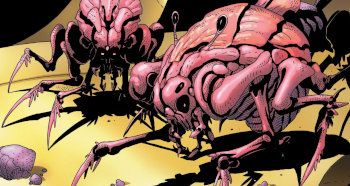
\includegraphics[width=\linewidth]{_img/bestiary/symbiote-abersyn.jpg}
\end{figure}